\documentclass[main.tex]{subfiles}

\begin{document}
\appendix
% Mental notat her på å fikse register map filene for fpga og mikrokontroller
\section{Software}

\subsection{Microcontroller Register Map}
\label{appendix: register_map}
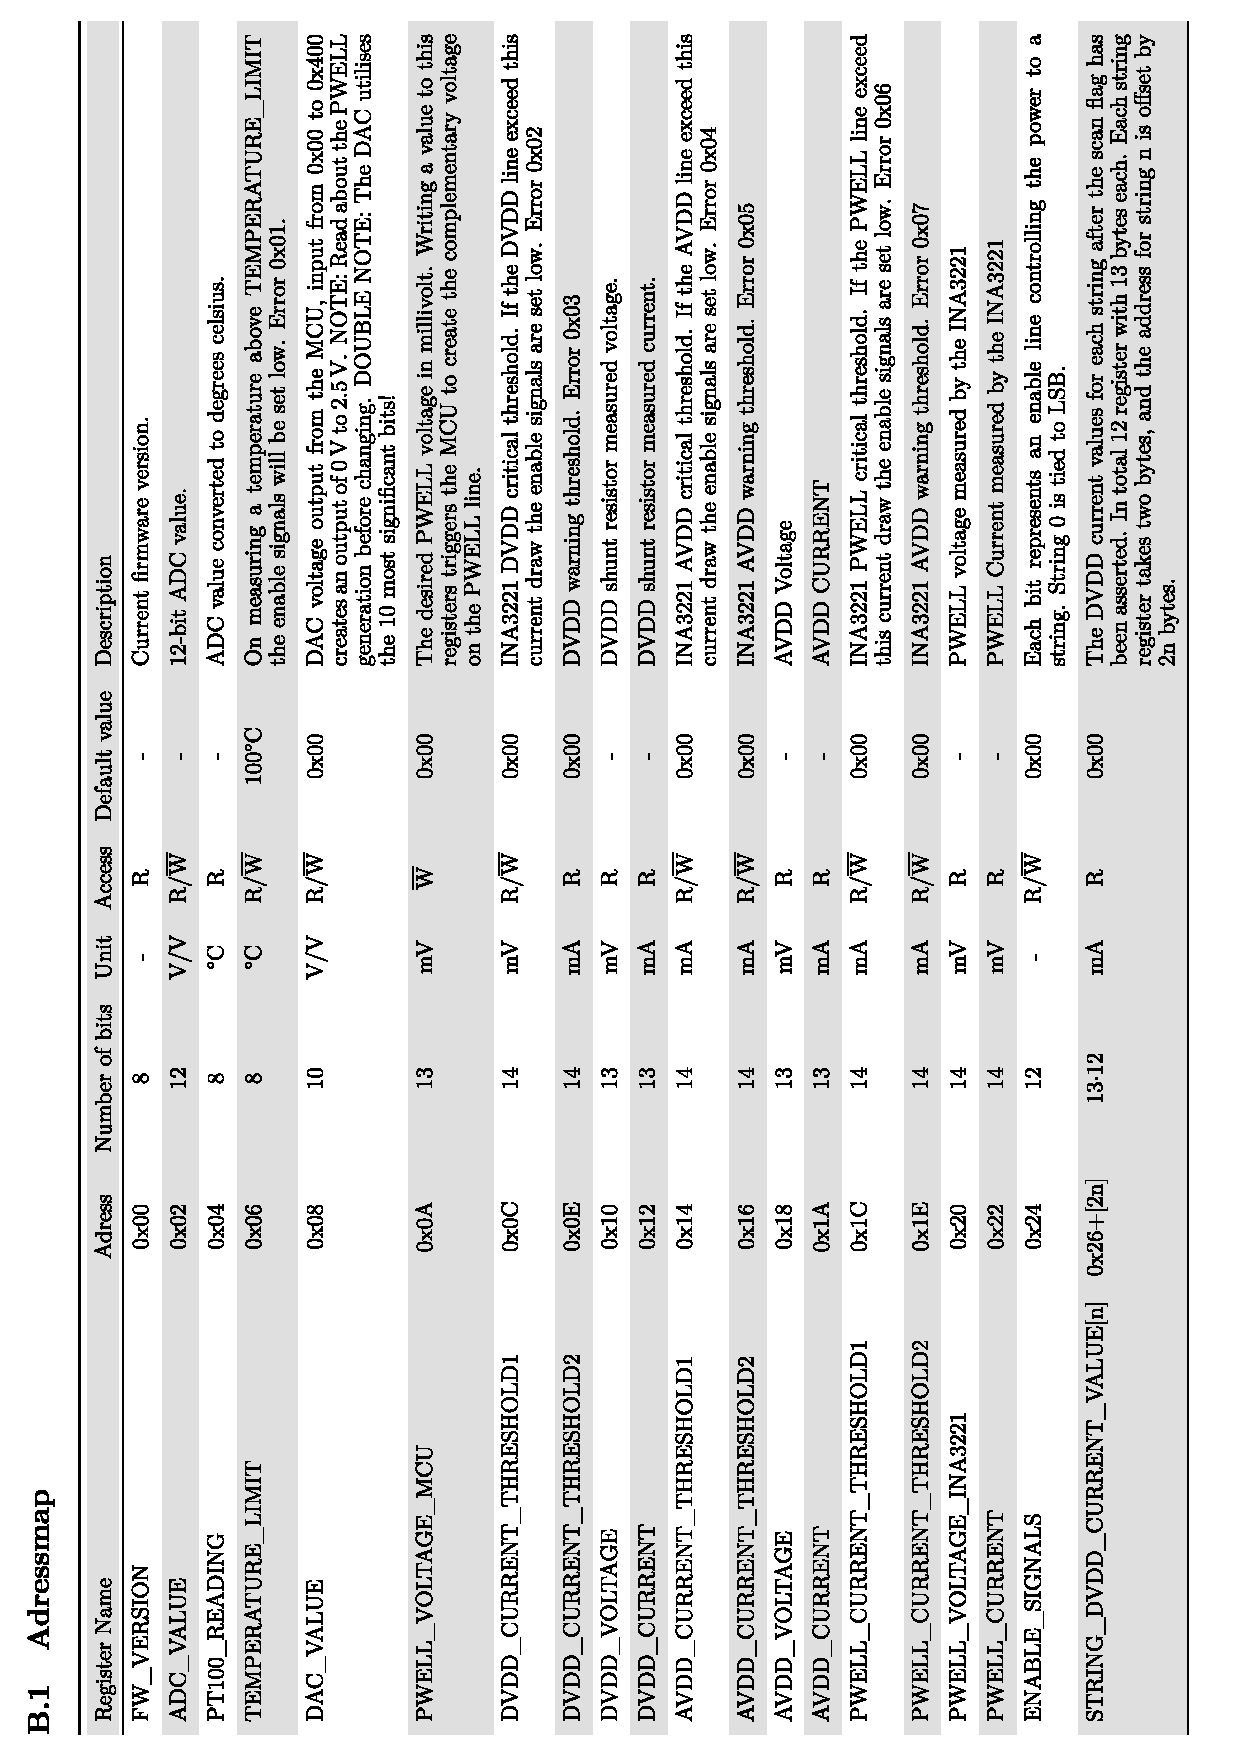
\includepdf{images/BITMAP.pdf}


\subsection{FPGA register map}
\label{appendix: fpga_map}
\begin{figure}[!htpb]
    \centering
    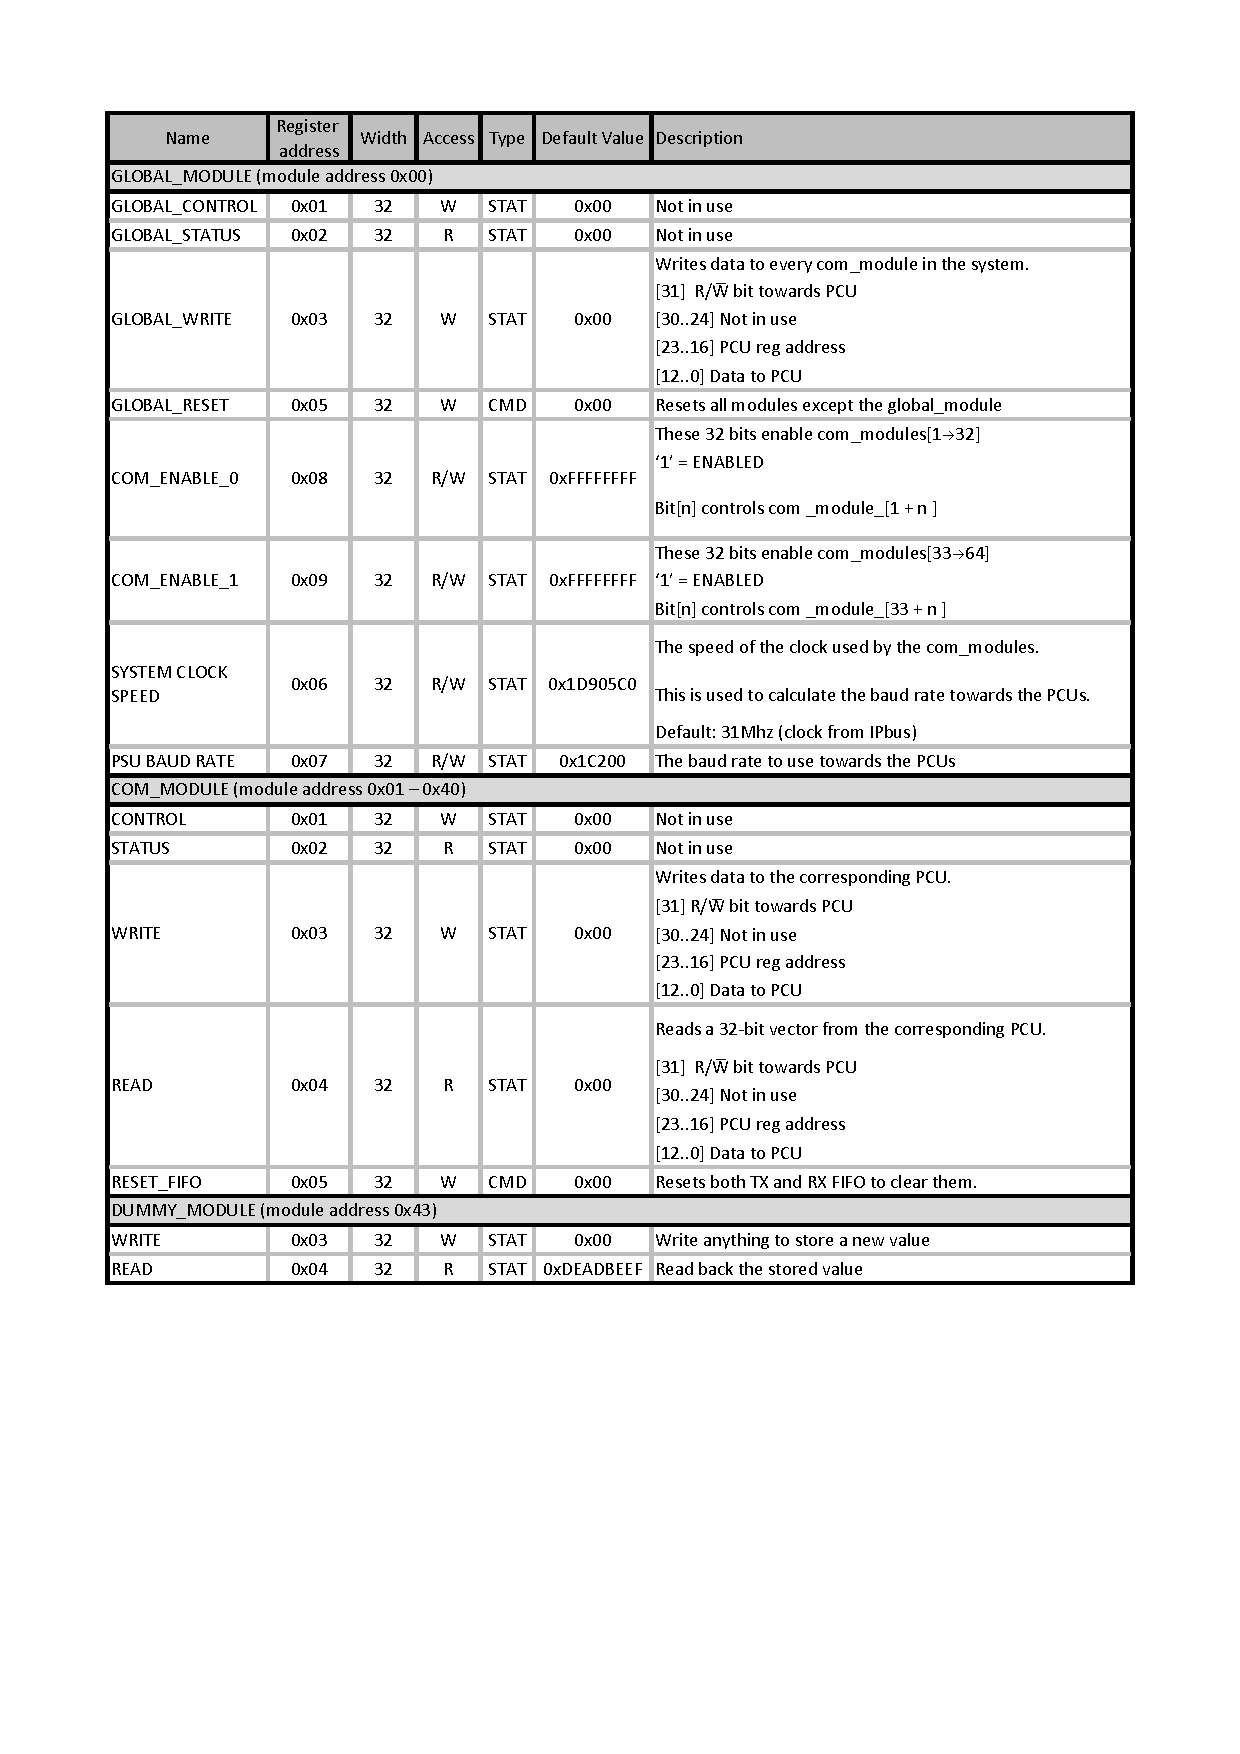
\includegraphics[ scale=1, height=25cm, width=20cm]{images/fpga_map.pdf}
\end{figure}
\FloatBarrier
\newpage

\section{Setting the Environment}

The control software is made of many libraries and programs that work together, this section will describe how to install and set up all dependencies involved in the \gls{pcs}.

\subsection{Python libraries}

The Python programs uses several libraries for communication and to process data. most of these can be installed using pip, but some require more setup. The following libraries are required:
\subsubsection{Bitstream}
Bitstream, used to perform bitwise operations on data from FPGA. Can be installed with:
\begin{verbatim}
pip install bitstream    
\end{verbatim}

\subsubsection{Qt5 Designer}
Qt5 designer, GUI program to design custom GUIs, installed with:

\begin{verbatim}
    sudo apt-get install qttools5-dev-tools
    sudo apt-get install qttools5-dev
\end{verbatim}
the program can then be opened with the command:
\begin{verbatim}
    designer
\end{verbatim}

The program creates .ui files which can be converted to python files using the command:

\begin{verbatim}
    pyuic5 -o example_gui.py example_gui.ui
\end{verbatim}

First parameter after -o is the name of the python file to be created and the second parameter is the name of the .ui file to be converted.

\subsubsection{pyMongo}
pyMongo is the \gls{api} between the python programs and the Mongo database. Can be installed with:

\begin{verbatim}
    pip install pymongo
\end{verbatim}

\subsubsection{InfluxDB}

InfluxDB is a time series database used for the monitoring system. They provide several different local versions depending on the operating system. They can be found here:
\begin{verbatim}
    https://portal.influxdata.com/downloads/
\end{verbatim}

For this project, the linux binaries option was used to install the database:
\begin{verbatim}
wget https://dl.influxdata.com/influxdb/releases/influxdb2-2.4.0-linux-amd64.tar.gz
tar xvfz influxdb2-2.4.0-linux-amd64.tar.gz
\end{verbatim}

The influx database can then be started with the command:

\begin{verbatim}
    influxd
\end{verbatim}

Influx is by default on port 8086 on localhost.

\subsubsection{Influx Python Client}
The InfluxDB client for Python. \gls{api} for writing and reading data to the Influx database using python. Can be installed with:

\begin{verbatim}
    pip install influxdb-client
\end{verbatim}

the Python client will need an \gls{api} token to connect to the database, this can be retrieved from the Influx web interface, in the data section, under python client library. This page also contains examples of various operations one can perform with the Influx python \gls{api}.

\section{Typical errors}

This section will cover common mistakes and pitfalls while using the software described in this thesis. Some may appear obvious, but it is documented here for the sake of completeness.

\subsection{Bit Error Rate and Masking}

The repository contains 3 tests for testing bit error rate in the transmission from control software to microcontroller, and back. These tests uses the microcontroller \gls{api} class when transmitting data, and the \gls{api} masks the data received, only keeping the data bits. One must disable the masking done in the microcontroller \gls{api} before performing these tests or the address and RnW bits will always turn out erroneous in the tests.

\subsection{InfluxDB Retention Policy}

The Influx web interface allows for setting the retention policy of the buckets in the database. The retention policy determines how long the database should bookkeep the data points from the monitoring process. There is also an option to not have a retention on the database, meaning it will store data points indefinitely. Storing the data points indefinitely can lead to a storage space problem, where one cannot boot up the server due to memory limits. There is no easy, immediate fix to this, I was not able to find a way to delete the data points, the "easiest" solution found was to re-install InfluxDB. There likely exist command lines that can fix this problem, but we could not find one while trying to fix this issue.

To avoid this issue altogether, always make sure that there is a set retention policy for every bucket in InfluxDB. The retention policies can be manually set through the Influx web interface.

\subsection{Bitstream}

"Bitstream" is a Python library used for performing bit wise operations on the data sent and retrieved in the \gls{pcs}-chain. It is primarily used to go through each bit of a bitstream, and it works by defining a bitstream object with a set bit-length and value. For whatever reason, if the bit-length is exactly high enough for the value inserted, the object will complain that the value is too high for the given bit length, i.e. it will return an error if the bit length is 3 and the inserted value is 5(0b101). Solution to this was to set the bit-length to be one more than what is needed, i.e. if a 32 bit vector must be analyzed, the length of the vector is set to 33. The consequence of the extra bit length is that each Bitstream will have a leading zero.

Bitstream works by having a pointer that starts at the \gls{msb}, and when reading one bit, the pointer moves to the next bit in the stream. The leading zero in the Bitstream can therefore be circumvented by performing an initial read to move the pointer past the leading zero before starting the bitwise operations.

\subsection{IPbus Address Values}

The IPbus address values are set in the XML-files, which determines the address value for the modules, as well as the addresses inside said modules. An unusual bug was discovered while testing the IPbus system using a dummy module. The first was that performing write requests to module 10 would also perform the same operation to module 1. Writing to module 12 would also write to module 2, and so on.

The cause for this was found to be the address values to each module. Module 1 had address 0x01, module 2 had 0x02, and so on, until module 10, which had address 0x10. I forgot while making the address values that these were hexadecimal values, not decimals, so I skipped straight to 0x10. In theory this should not have an effect on anything in the IPbus system, all that is important is that the address values are unique, but in this instance, changing module 10 to have address 0x0A fixed the problem. The underlying cause of this issue was never discovered, so efforts should be made to ensure that address values are sequential and consistent.

The cause of the bug was not determined, but the fault could have been in the use of the dummy module, which served as a hardware simulator.

\subsection{Grafana}

Setting up graphs and queries in Grafana can be time consuming and performing operations on all 43 displays on the dashboard is very repetitive and inefficient. A more efficient way of modifying the dashboard in any capacity is to not to directly use the Grafana dashboard. Instead, download the JSON-format of the dashboard, this can be accessed by going into the settings menu on a specific dashboard. Then go to "JSON Model" and copy the the code there. Put the code in a text editor, such as Visual Studio Code, and manipulate the dashboard from there. Changing variable names or query request of multiple graphs can be done relatively easy using this method.

When done editing the file, go to the Dashboard menu on the Grafana web interface and click import:

\begin{figure}[!ht]
    \centering
    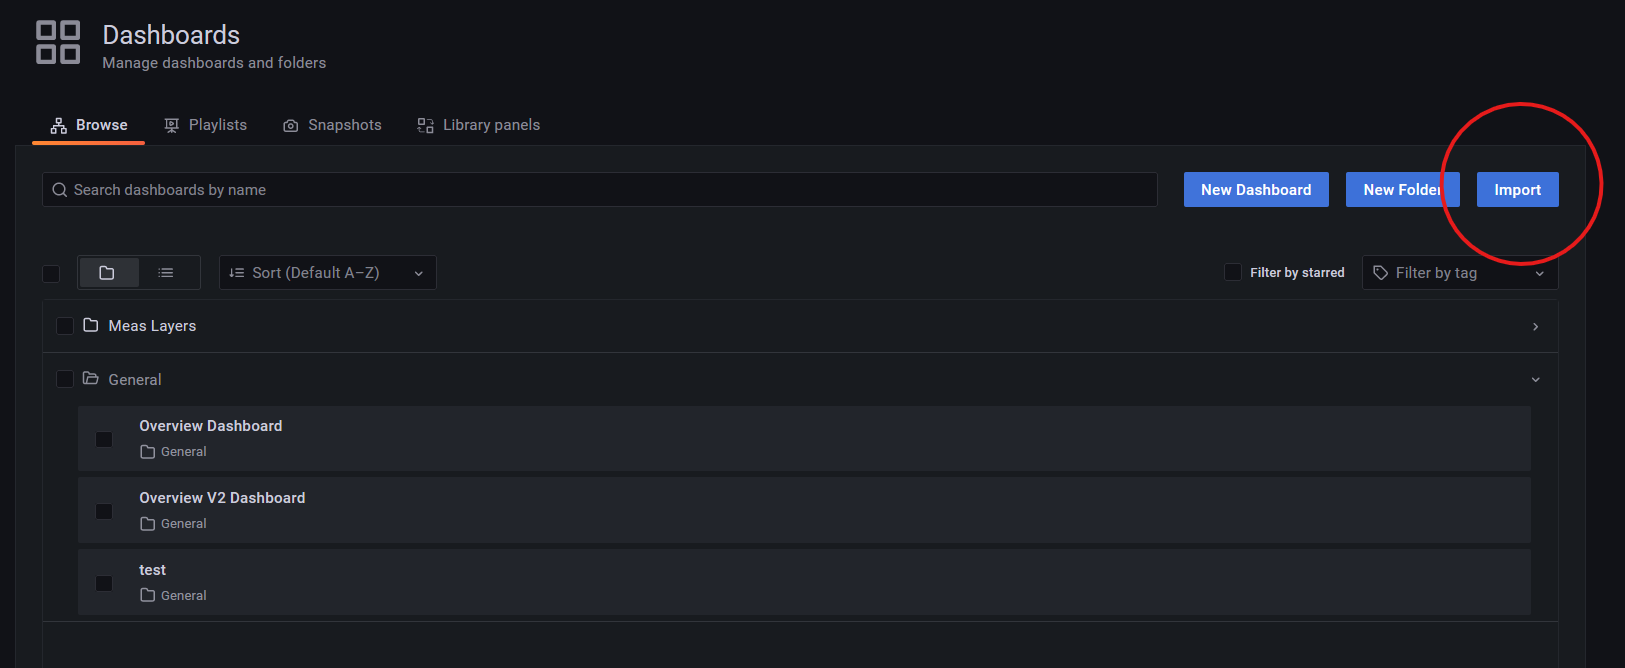
\includegraphics[scale=0.4]{images/grafana_import.png}
    \caption{Grafana dashboard highlighting the import button.}
    \label{fig: grafana_import}
\end{figure}
\FloatBarrier 

From there enter your edited JSON-file and create the new dashboard, note that it will require a different ID value than the dashboard it was copied from.


\subsection{FPGA FIFOs}

Strange behaviour was detected in the \gls{fpga} design whenever an attempt was made to read from an already empty FIFO. This behaviour added seemingly random values into the \gls{fifo}s while performing read and write requests. This bug should be fixed in the latest version of the bit-file for the \gls{fpga}, but to ensure consistency in the tests of the \gls{pcs}-chain, a check is done in the tests to ensure that we are not reading an empty \gls{fifo}. The tests check if received data is equal to zero, if it is, then the \gls{fifo} was read too soon. This may happen if the \gls{fpga} does not get a response from the microcontroller in time or if the baud rate is too low compared to the speed of the read/write requests from the control software.

Also important to note, if the \gls{fifo} was read too soon, then the rest of the transmissions will fall out of synch and will not match the expected result, and then the entire test is invalid. That is also why it is important to perform a reset of the modules for each test performed, to ensure that all \gls{fifo}s are empty when starting a new test.

\notinmain{IPbus/uhal, mongoDB(sjekk mer opp i denne, alternativt bare bruk Jonas sin install commands), pyMongo, influxdb, influxdb pytohn client, telegraf plugin, grafana}


\end{document}